\subsection{Validation of the photoproduction trigger}

As described in section \ref{sec:photoproduction_trigger}, the CLAS12 photoproduction trigger requires the coincidence between one electron measured in the Forward Tagger detector, and two hadrons measured within the CLAS12 detector, in the forward or central part. The validation procedure aims to verify if, for a given event foreseeing one final-state electron in the FT acceptance and two or more hadrons scattered within the CLAS12 acceptance, the trigger system would recognize it properly, resulting in event readout. In order to validate the system with beam during commissioning, the following strategy was adopted. First, the $e^-$ detection by the FT was validated using Random Trigger runs. After this, the detection of single hadrons in CLAS12 was studied in special runs, were the only trigger source was the FT. Finally, the coincidence between the two systems was assessed.

\subsubsection{Validation of $e^-$ detection in FT}

A scattered electron in the Forward Tagger is identified as an electromagnetic shower in the Forward Tagger Calorimeter within a proper energy range, in time coincidence and geometrically matched to a hit in both layers of the Forward Tagger Hodoscope. The map providing the matching between the cluster seed position in the FT-Cal and the tiles position in the FT-Hodo was first derived by the nominal detector geometry, and then confirmed by Montecarlo simulations.

The identification of the scattered $e^-$ in the FT was validated through a similar procedure as the one adopted for the CLAS12 electron trigger discussed before, based on ``Random Trigger'' runs. Recorded events were processed through the standard CLAS12 reconstruction software and filtered, keeping only those with a reconstructed $e^-$ in the FT system. Since event readout was triggered by a random pulser, events with the reconstructed $e^-$ signal close to the margins of the readout window were also rejected.
For these events, the electromagnetic clusters found by the reconstruction software (``offline'' clusters) were compared to those reported by the trigger system and stored in the form of the trigger data banks.

The efficiency of the FT-Cal clustering algorithm in the trigger system was evaluated by comparing all ``offline'' clusters to those matched - in space and time - to an ``online'' one\footnote{The energy of ``offline'' clusters is properly corrected to account for electromagnetic shower leakage from the bak of the FT-Cal, while ``online'' clusters do not implement this. Therefore, for a given $e^-$ in the FT-Cal, there is a systematic difference between the two energies. This effect is properly taken into account when setting the energy range for $e^-$ detection in the trigger system, and does not affect the corresponding trigger efficiency.}. The efficiency was computed as:
\begin{equation}
\varepsilon=\frac{N_{trigger}}{N_{all}} \; ,
\end{equation}
where $N_{all}$ and $N_{trigger}$ are, respectively, the total number of ``offline'' clusters and the number of ``offline'' clusters matched to an ``online'' one.
The result is shown in Fig.~\ref{fig:FT_ClusterEfficiency}, reporting the FT trigger efficiency for electromagnetic clusters as a function of the corresponding corrected energy. Efficiency is higher than 97.5$\%$ in the full energy range of interest / 99.5$\%$ in the energy range above 1 GeV. The difference is mainly due to the fact that the clustering algorithm in the trigger system works on a 3x3 matrix of crystals, whereas this limitation doesn't hold in the offline reconstruction.
The efficiency of the FT-Cal / FT-Hodo matching algorithm was evaluated in a similar way, repeating previous calculation but considering only electromagnetic clusters associated to one hit in each FT-Hodo layer. The result is reported in Fig.~\ref{fig:FT_ClusterEfficiencyHODO}.

%%%%%%%%%%%%%%%%%%%%%%%%%%%%%%%%%%%%%%%%% F I G U R E %%%%%%%%%%%%%%%%%%%%%%%%%%%%%%%%%%%%%%%%%%
\begin{figure}[!htb]
 \centering
{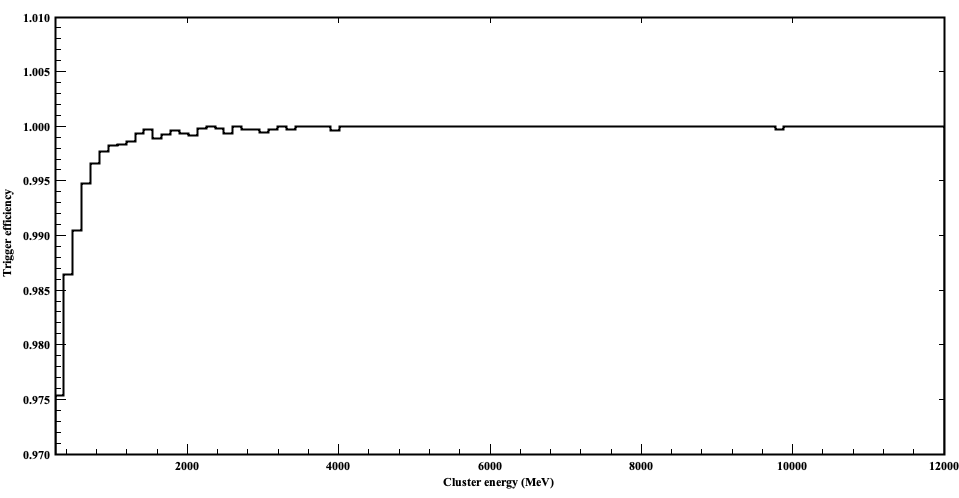
\includegraphics[width=.5\textwidth]{img/FT_ClusterEfficiency.png}}
 \caption{TODO: better figure, with errors (run 4288)}
 \label{fig:FT_ClusterEfficiency}
\end{figure}
%%%%%%%%%%%%%%%%%%%%%%%%%%%%%%%%%%%%%%%%% F I G U R E %%%%%%%%%%%%%%%%%%%%%%%%%%%%%%%%%%%%%%%%%%




\subsubsection{Validation of charged hadrons detection in CLAS12-FD}

The trigger system recognizes a charged hadron in the CLAS12 forward detector as a hit in the Forward Time-Of-Flight system (panel 1B) in time coincidence and geometrically matched to a hit in the U-bars of the Preshower Calorimeter, associated to a cluster with energy larger than a programmable threshold. The map providing the geometrical matching between FTOF counter and the PCAL U-bar was first derived by the nominal detector geometry, and then confirmed by Montecarlo simulations. To reduce the rate of random coincidences, the trigger system also requires the presence of a segment in 5 out of 6 drift chamber layers. The charged hadron identification algorithm was validated in special data-taking runs in which the Forward Tagger was the only enabled event readout source. In these runs, the trigger system was configured to report in the output trigger bank the presence of a charged hadron in any CLAS12-FD sector, as defined before. 

Recorded events were processed through standard reconstruction software and filtered, keeping only those with a well reconstructed charged track measured in CLAS12-FD. The track was required to be within the nominal acceptance of CLAS12 PCAL, and a momentum threshold of 300 MeV/c was applied. The trigger system efficiency was evaluated by comparing all reconstructed tracks to the tracks recognized by the trigger system. During commissioning, the efficiency was evaluated as a function of different observables, such as the energy deposited in the FTOF counters and in the PCAL, and the topology of the geometrical matching window. Trigger parameters were individually tuned to maximize the trigger efficiency. In the final configuration, an energy threshold of 2 MeV and 10 MeV for the FTOF counters and PCAL clusters was selected.  The result is reported in Fig.~\ref{fig:FD_TrackEfficiency}, showing the CLAS12-FD trigger efficiency for charged hadrons as a function of the track momentum. The efficiency is larger than 99$\%$ in the full momentum range, the inefficiency being dominated by threshold effects for the PCAL clusters.

%%%%%%%%%%%%%%%%%%%%%%%%%%%%%%%%%%%%%%%%% F I G U R E %%%%%%%%%%%%%%%%%%%%%%%%%%%%%%%%%%%%%%%%%%
\begin{figure}[!htb]
 \centering
{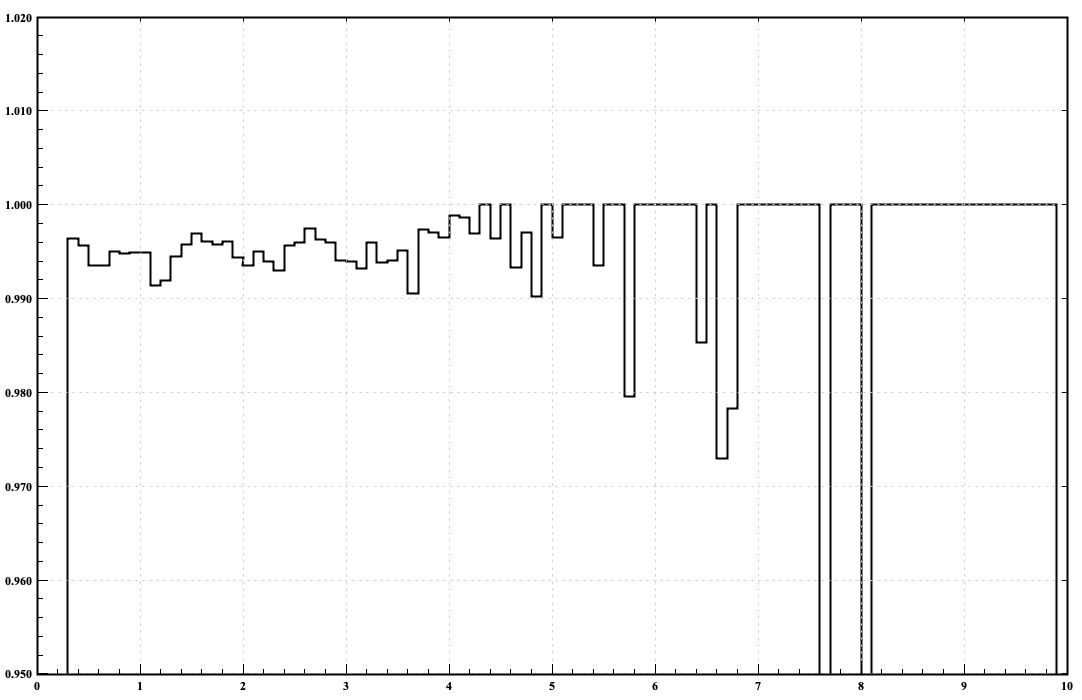
\includegraphics[width=.5\textwidth]{img/FD_TrackEfficiency.png}}
 \caption{TODO: better figure, with errors - run 5049-5050 (run4)}
 \label{fig:FD_TrackEfficiency}
\end{figure}
%%%%%%%%%%%%%%%%%%%%%%%%%%%%%%%%%%%%%%%%% F I G U R E %%%%%%%%%%%%%%%%%%%%%%%%%%%%%%%%%%%%%%%%%%



\subsubsection{Validation of charged hadron detection in CLAS12-CD}

The trigger system recognizes a charged hadron in the CLAS12 central detector as a hit in the Time-Of-Flight system (panel 1B) in time coincidence and geometrically matched to a hit in the U-bars of the Preshower Calorimeter.

